\chapter{Resultados}
\label{resultados}

En este capítulo mostramos todos los resultados obtenidos, tanto del entrenamiento con imágenes sintéticas como con imágenes SAR reales. Presentamos también todos los métodos de medición de la calidad del modelo, desde el mismo error de validación hasta métodos estadísticos y la comparación con otros filtros.

\section{Modelos entrenados con imágenes sintéticas}

Empezamos analizando los modelos que entrenamos utilizando las imágenes sintéticas creadas de la forma descrita en la sección \ref{sec:construccion_imagenes_SAR}.

\subsection{Arquitecturas}

\titulito{Metodología de diseño}

En el desarrollo de las arquitecturas de autoencoders convolucionales para este trabajo seguimos una metodología sistemática de exploración y refinamiento progresivo. La estrategia adoptada consistió en comenzar con arquitecturas base simples y agregar complejidad de manera controlada. Cabe destacar la dificultad que presentan los modelos de redes neuronales al no permitir la optimización de hiperparámetros. Como la misma arquitectura puede variar, incluyendo la cantidad y tipo de capas, no es factible buscar los parámetros óptimos con los métodos tradicionales. O al menos no lo es si no se posee un poder de computo muy elevado.

El conjunto total de $25$ configuraciones que desarrollamos puede clasificarse en cinco categorías principales, cada una diseñada para investigar aspectos específicos del modelo: arquitecturas base o de referencia, variaciones sistemáticas de la profundidad de la red, estudios de dimensionalidad del espacio latente, análisis del efecto de la duración del entrenamiento, y experimentos con configuraciones especiales y atípicas.

En lo que sigue hablaremos de algunas de las arquitecturas principales. Pero en la tabla \ref{tab:autoencoder_configs} las resumimos a todas.

\begin{table}[htbp]
\centering
\caption{Resumen de todas las configuraciones de redes neuronales convolucionales que diseñamos en este trabajo.}
\label{tab:autoencoder_configs}
\scriptsize
\begin{tabular}{|c|c|c|c|c|c|c|}
\hline
\textbf{Config.} & \textbf{Capas Conv.} & \textbf{\emph{Encoding Dim.}} & \textbf{Épocas} & \textbf{Muestras} & \textbf{LR} & \textbf{\emph{Scheduler}} \\
\hline
\hline
\multicolumn{7}{|c|}{\textbf{Arquitecturas Base y de Referencia}} \\
\hline
A1 & 1+\emph{MaxPool} & 32 & 5 & 50K & 0.001 & Ninguno \\
A2 & 1 & 32 & 30 & 50K & 0.001 & ELR \\
A3 & 2+\emph{MaxPool} & 512 & 500 & 50K & 0.001 & ELR \\
\hline
\hline
\multicolumn{7}{|c|}{\textbf{Variaciones por Profundidad}} \\
\hline
\multicolumn{7}{|c|}{\textit{1 Capa Convolucional}} \\
\hline
A4 & 1 & 32 & 500 & 50K & 0.001 & Ninguno \\
A5 & 1 & 32 & 70 & 50K & 0.001 & Ninguno \\
A6 & 1 & 32 & 500 & 50K & 0.0005 & Ninguno \\
\hline
\multicolumn{7}{|c|}{\textit{2 Capas Convolucionales}} \\
\hline
A7 & 2 & 128 & 500 & 50K & 0.001 & ELR \\
A8 & 2 & 128 & 70 & 50K & 0.001 & ELR \\
A9 & 2 & 256 & 500 & 50K & 0.001 & ELR \\
A10 & 2 & 256 & 70 & 50K & 0.001 & ELR \\
A11 & 2 & 64 & 100 & 100K & 0.001 & RLROP \\
A12 & 2 & 64 & 40 & 100K & 0.001 & RLROP \\
\hline
\multicolumn{7}{|c|}{\textit{3+ Capas Convolucionales}} \\
\hline
A13 & 3 & 128 & 500 & 50K & 0.001 & ELR \\
A14 & 3 & 128 & 70 & 50K & 0.001 & ELR \\
A15 & 3 & 256 & 500 & 50K & 0.001 & ELR \\
A16 & 3 & 256 & 70 & 50K & 0.001 & ELR \\
A17 & 3+Densa & 128 & 500 & 50K & 0.001 & Ninguno \\
A18 & 3+Densa & 128 & 70 & 50K & 0.001 & Ninguno \\
A19 & 3 & 64 & 100 & 100K & 0.001 & RLROP \\
A20 & 4+Densa & 64 & 100 & 100K & 0.001 & RLROP \\
\hline
\hline
\multicolumn{7}{|c|}{\textbf{Entrenamientos Especiales}} \\
\hline
A21 & 1 & 32 & 15 & 50K & 0.001 & ELR \\
A22 & 1 & 32 & 500 & 50K & 0.001 & ELR \\
A23 & 1 & 32 & 500 & 100K & 0.001 & ELR \\
\hline
\hline
\multicolumn{7}{|c|}{\textbf{Arquitecturas Experimentales}} \\
\hline
A24 & Conv2DT* & 32 & 20 & 50K & 0.001 & Ninguno \\
A25 & Conv2DT* & 32 & 11 & 50K & 0.001 & Ninguno \\
\hline
\end{tabular}

\begin{flushleft}
\footnotesize
\textbf{Notas:}
\begin{itemize}
    \item \textbf{\emph{Encoding dim.}}: Dimensión más pequeña de la red, es la dimensión de la capa intermedia
    \item \textbf{Muestras}: Tamaño del dataset usado para entrenar
    \item \textbf{LR}: \emph{Learning Rate}
    \item \textbf{ELR}: \emph{Exponential Learning Rate} ($\gamma=0.95$)
    \item \textbf{RLROP}: \emph{Reduce Learning Rate on Plateau} ($factor=0.8$)
    \item \textbf{Conv2DT*}: Usa convolución traspuesta en el encoder (arquitectura atípica)
    \item Todos los modelos usan: Optimizador Adam, MSE de función de pérdidas, \emph{Batch size} de 64
    \item Activaciones: ReLU (capas ocultas), Sigmoidea (salida)
\end{itemize}
\end{flushleft}
\end{table}

\titulito{1 - Arquitecturas base o de referencia}

La primera categoría establece los fundamentos arquitectónicos del trabajo mediante tres configuraciones que exploran diferentes enfoques. En la configuración A1 implementamos un diseño tradicional que combina una capa convolucional inicial con \emph{max-pooling} para la reducción dimensional, seguido de capas densas para la codificación. Esta arquitectura representa el enfoque clásico donde la extracción de características convolucionales se combina con representación densa en el cuello de botella.

En la configuración A2 introducimos el concepto de simetría arquitectónica, utilizando convoluciones con \emph{stride} para la reducción dimensional en lugar de \emph{pooling} explícito. Esta aproximación mantiene la coherencia entre las operaciones del encoder y decoder, donde las convoluciones con \emph{stride} se corresponden directamente con convoluciones transpuestas para la reconstrucción. La simetría es un principio fundamental en el diseño de autoencoders, ya que facilita la reversibilidad de las transformaciones aplicadas a los datos.

En la tercera configuración de referencia, A3, combinamos operaciones de \emph{max-pooling} con \emph{upsampling}, representando un enfoque híbrido que utiliza diferentes mecanismos para la reducción y expansión dimensional. En esta configuración también empleamos un espacio latente significativamente mayor ($512$ dimensiones), explorando el efecto de una representación intermedia más rica.

\titulito{2 - Variaciones sistemáticas de la profundidad de la red}

La segunda categoría constituye el núcleo del análisis arquitectónico, organizando las configuraciones según el número de capas convolucionales para estudiar sistemáticamente el efecto de la profundidad en el rendimiento del modelo. Esta categorización permite evaluar cómo la capacidad de extracción de características jerárquicas impacta en la calidad de la reconstrucción.

\begin{itemize}
    \item \emph{Arquitecturas de una capa convolucional}

    En las arquitecturas más simples utilizamos una única capa convolucional para la extracción de características. La configuración A2 sirve como referencia principal, implementando un encoder con una capa convolucional seguida de aplanamiento y una capa densa. En las variantes A4 y A6 mantenemos esta arquitectura base pero exploran diferentes tasas de aprendizaje, investigando si la simplicidad arquitectónica puede compensarse con ajustes en la optimización.
    
    Estas arquitecturas representan el caso mínimo viable para un autoencoder convolucional, donde la extracción de características se limita a patrones locales de bajo nivel. Nuestra expectativa es que estas configuraciones puedan ser suficientes para datos con estructura simple pero muestren limitaciones con patrones más complejos.
    
    \item \emph{Arquitecturas de dos capas convolucionales}
    
    La expansión a dos capas convolucionales nos permite la captura de características de mayor nivel de abstracción. En las configuraciones A7 y A9 implementamos esta arquitectura con diferentes dimensiones del espacio latente ($128$ y $256$ respectivamente), permitiendo evaluar simultáneamente el efecto de la profundidad y la capacidad del cuello de botella.
    
    Las configuraciones A11 y A12 representan una variante especializada dentro de esta categoría, utilizando \emph{padding} agresivo y un dataset expandido ($100.000$ muestras frente a las $50.000$ que usualmente utilizamos en las arquitecturas anteriores). Las diseñamos específicamente para evaluar el rendimiento en condiciones de datos abundantes. Es útil destacar que no tenemos inconvenientes en armar un dataset grande dado que lo generamos nosotros mismos artificialmente. Pero tener una cantidad muy extensa de imágenes para procesar nos obstaculiza en cuanto extiende mucho el tiempo de entrenamiento.
    
    La progresión de filtros típica en estas arquitecturas ($8\rightarrow 16$ o $32\rightarrow 64$) sigue el principio establecido en redes convolucionales donde el número de filtros aumenta mientras las dimensiones espaciales se reducen, permitiendo que el modelo capture gradualmente características más abstractas y globales.
    
    \item \emph{Arquitecturas de tres o más capas convolucionales}
    
    Con las arquitecturas más profundas exploramos la capacidad de extracción jerárquica de características complejas. En las configuraciones A13 y A15 implementamos tres capas convolucionales con progresión $8\rightarrow 16\rightarrow 32$ filtros, nuevamente variando la dimensión latente para un análisis completo.
    
    En la configuración A17 introducimos complejidad adicional mediante una capa densa intermedia en el encoder después del aplanamiento, representando un híbrido entre enfoques puramente convolucionales y densos. Con esta arquitectura investigamos si capas densas adicionales pueden mejorar la representación antes de la compresión final al espacio latente.
    
    Las configuraciones con mayor cantidad de parámetros ajustables incluyen A19 (tres capas: $32\rightarrow 64\rightarrow 128$) y A20 (cuatro capas más una capa densa intermedia). Estas representan los modelos más complejos del estudio y los diseñamos para evaluar el límite superior del rendimiento alcanzable con la metodología propuesta y los recursos de tiempo y computo disponibles.

\end{itemize}

\titulito{3 - Estudios de dimensionalidad del espacio latente}

La dimensión del espacio latente representa un parámetro crítico que controla el equilibrio entre compresión y capacidad de representación. Las configuraciones las distribuimos estratégicamente a través de diferentes dimensiones latentes para caracterizar esta relación.

Las configuraciones con $32$ dimensiones (A2, A4, etc.) representan alta compresión, forzando al modelo a aprender representaciones muy eficientes pero potencialmente limitadas. Las configuraciones con $64$ dimensiones (A19, A11, A20) proporcionan un equilibrio intermedio, mientras que aquellas con $128$ y $256$ dimensiones permiten representaciones más ricas a costa de menor compresión.

La configuración A3 con $512$ dimensiones representa el extremo de baja compresión, investigando si espacios latentes muy grandes pueden mejorar la calidad de reconstrucción cuando la compresión no es prioritaria.

\titulito{4 - Análisis del efecto de la duración del entrenamiento}

Una característica del diseño experimental que construimos es la inclusión sistemática de pares de configuraciones idénticas que difieren únicamente en el número de épocas de entrenamiento. Este enfoque nos permite evaluar si las diferencias de rendimiento entre arquitecturas se deben a limitaciones estructurales o simplemente a entrenamiento insuficiente.

Los pares incluyen comparaciones desde entrenamientos cortos (entre $11$ y $15$ épocas) hasta entrenamientos extensos (alrededor de $500$ épocas), cubriendo arquitecturas simples hasta otras complejas. Esta metodología es valiosa porque permite distinguir entre:

\begin{itemize}
    \item Limitaciones arquitectónicas fundamentales: Cuando incluso entrenamientos largos no mejoran el rendimiento.
    \item Necesidades de optimización diferentes: Cuando arquitecturas complejas requieren más tiempo para converger.
    \item Sobreajuste (o \emph{overfitting}): Cuando entrenamientos largos, aunque generan mejores errores durante el entrenamiento, degradan el rendimiento en validación. El modelo aprende a representar con demasiado detalle el dataset de entrenamiento, a costa de generalizar.
\end{itemize}

\titulito{5 - Configuraciones especiales y experimentales}

\begin{itemize}
    \item \emph{Configuraciones con datos mixtos}

    En las configuraciones A23 y A20 utilizamos datasets que combinan diferentes particiones de imagen ($1\times 1$ y $2\times 2$ cuadrados, o $1\times 1$, $2\times 2$ y $3\times 3$ respectivamente). En estos experimentos evaluamos la capacidad de generalización de los modelos cuando se entrenan con datos de diferente granularidad espacial. Se espera que esta metodología les permita no aprender los bordes de una partición específica, lo cual correspondería a \emph{overfitting}.

    \item \emph{Arquitecturas experimentales atípicas}

    La configuración A24 representa un caso experimental deliberadamente atípico, utilizando una convolución traspuesta en el encoder (operación normalmente reservada para el decoder) seguida de \emph{max-pooling}. En el decoder utilizamos únicamente capas densas, creando una asimetría arquitectónica marcada. Esta configuración sirve como control negativo, investigando qué ocurre cuando violamos principios arquitectónicos establecidos para los autoencoders.
\end{itemize}

\titulito{Principios de diseño y progresión lógica}

La progresión de arquitecturas que construimos sigue varios principios de diseño establecidos en el campo:

\begin{enumerate}
    \item Incremento gradual de complejidad: Comenzando con una capa convolucional y aumentando sistemáticamente hasta cuatro capas.

    \item Simetría encoder-decoder: Manteniendo correspondencia entre operaciones de reducción y expansión dimensional.

    \item Progresión de filtros: Aumentando el número de filtros mientras reducimos las dimensiones espaciales.

    \item Control experimental: Manteniendo factores constantes (optimizador Adam, MSE como función de pérdida, activaciones ReLU/Sigmoidea) mientras variamos los aspectos arquitectónicos de interés.
\end{enumerate}

Esta metodología nos permite identificar tanto las componentes arquitectónicas más efectivas como las configuraciones que representan complejidad innecesaria, proporcionando una base para conclusiones sobre el diseño óptimo de autoencoders convolucionales para la reducción del ruido \emph{speckle}.

\subsection{Errores de entrenamiento y test}

En el cuadro \ref{tab:testing_results} presentamos los resultados del error de testeo para cada arquitectura, ordenados de mejor a peor rendimiento. Recordemos que ese error se calcula sobre un conjunto de $1000$ imágenes armadas artificialmente de la misma manera que el conjunto de entrenamiento. La tabla incluye tanto el error de test (MSE) como el error de entrenamiento en la última época, junto con el porcentaje de variación entre ambos (tomando como base al de entrenamiento). Este último indicador resulta fundamental para identificar posibles casos de \emph{overfitting}: porcentajes de aumento significativos del error de testeo respecto al de entrenamiento sugieren que el modelo ha perdido capacidad de generalización.

Aclaramos también que la configuración A3 no pudo entrenarse dada la gran cantidad de parámetros entrenables que poseía. Los recursos computacionales disponibles y el tiempo no fueron suficientes para este propósito.

\definecolor{rojito}{RGB}{255,150,150}
\definecolor{verdecito}{RGB}{10,255,100}

\begin{table}[htbp]
\centering
\caption{Resultados del error de testeo para cada configuración (ordenados por rendimiento), y el error de entrenamiento en la última época. También se muestra la variación del primero con respecto al segundo. Este valor es verde cuanto la variación es negativa, rojo cuando es positiva, y rojo más intenso cuando el aumento es mayor al 10\%.}
\label{tab:testing_results}
\footnotesize
\begin{tabular}{|c|c|c|c|c|}
\hline
\textbf{Ranking} &
\textbf{Config.} &
\makecell{\textbf{Error de} \\ \textbf{\emph{test} (MSE)}} &
\makecell{\textbf{Error de \emph{train} (MSE)} \\ \textbf{en la última época}} &
\makecell{\textbf{Error de \emph{test}} \\ \textbf{vs. \emph{train}}} \\
\hline
1 & A15 & 0.002319 & 0.002318 & \textcolor{rojito}{$\nearrow 0.04\%$} \\
2 & A13 & 0.002346 & 0.002412 & \textcolor{verdecito}{$\searrow 2.74\%$} \\
3 & A16 & 0.002348 & 0.002387 & \textcolor{verdecito}{$\searrow 1.63\%$} \\
4 & A7 & 0.002433 & 0.002318 & \textcolor{rojito}{$\nearrow 4.96\%$} \\
5 & A18 & 0.002485 & 0.002174 & \textcolor{red}{$\nearrow 14.31\%$} \\
6 & A14 & 0.002421 & 0.002380 & \textcolor{rojito}{$\nearrow 1.72\%$} \\
7 & A24 & 0.002505 & 0.002520 & \textcolor{verdecito}{$\searrow 0.60\%$} \\
8 & A10 & 0.002516 & 0.002313 & \textcolor{rojito}{$\nearrow 8.78\%$} \\
9 & A17 & 0.002528 & 0.002108 & \textcolor{red}{$\nearrow 19.92\%$} \\
10 & A9 & 0.002547 & 0.002283 & \textcolor{red}{$\nearrow 11.56\%$} \\
11 & A12 & 0.002575 & 0.002216 & \textcolor{red}{$\nearrow 16.20\%$} \\
12 & A25 & 0.002586 & 0.002566 & \textcolor{rojito}{$\nearrow 0.78\%$} \\
13 & A2 & 0.002594 & 0.002314 & \textcolor{red}{$\nearrow 12.10\%$} \\
14 & A8 & 0.002568 & 0.002383 & \textcolor{rojito}{$\nearrow 7.76\%$} \\
15 & A11 & 0.002643 & 0.002197 & \textcolor{red}{$\nearrow 20.30\%$} \\
16 & A4 & 0.002781 & 0.002164 & \textcolor{red}{$\nearrow 28.51\%$} \\
17 & A22 & 0.002799 & 0.002245 & \textcolor{red}{$\nearrow 24.68\%$} \\
18 & A5 & 0.002879 & 0.002774 & \textcolor{rojito}{$\nearrow 3.79\%$} \\
19 & A6 & 0.003444 & 0.002666 & \textcolor{red}{$\nearrow 29.18\%$} \\
20 & A20 & 0.003691 & 0.003071 & \textcolor{red}{$\nearrow 20.19\%$} \\
21 & A21 & 0.004343 & 0.004349 & \textcolor{verdecito}{$\searrow 0.14\%$} \\
22 & A19 & 0.005331 & 0.005353 & \textcolor{verdecito}{$\searrow 0.41\%$} \\
23 & A1 & 0.005695 & 0.005349 & \textcolor{rojito}{$\nearrow 6.47\%$} \\
24 & A23 & 0.011212 & 0.011238 & \textcolor{verdecito}{$\searrow 0.23\%$} \\
\hline
- & A3 & - & - & - \\
\hline
\end{tabular}

\vspace{0.5cm}

\begin{flushleft}
\footnotesize
\textbf{Nota:}
La configuración A3 no presenta datos porque no pudimos llevar a cabo el entrenamiento ya que los parámetros entrenables eran demasiados y el poder de computo disponible no era suficiente.
\end{flushleft}
\end{table}

\titulito{Arquitecturas con Mejor Rendimiento}

Las tres mejores configuraciones corresponden a arquitecturas de tres capas convolucionales: A15, A13 y A16. Estas arquitecturas logran errores de testing entre $0.002319$ y $0.002348$, estableciendo claramente que la profundidad arquitectónica combinada con dimensiones latentes elevadas ($128$-$256$) constituye la estrategia más efectiva para este dominio de aplicación. Además, en los tres casos el error de testeo es muy similar al de entrenamiento, indicando excelente capacidad de generalización sin sobreajuste significativo.

Particularmente notable es el rendimiento de A16, que con solo $70$ épocas de entrenamiento alcanza el tercer lugar, sugiriendo que estas arquitecturas profundas convergen rápidamente hacia soluciones óptimas. El error de A16 es solo marginalmente mayor al de A15 y A13.

\titulito{Arquitecturas con \emph{overfitting}}

Varias configuraciones exhiben indicios de sobreajuste. La más grave de todas siendo la configuración A6 con un aumento del $29.18\%$ en el error de testeo respecto al de entrenamiento, seguida de A4 con un incremento del $28.51\%$. Estos casos sugieren que los modelos han memorizado patrones específicos del conjunto de entrenamiento sin desarrollar representaciones generalizables.

Son $10$ las arquitecturas totales que presentan un error de testeo al menos un $10\%$ más grande que el de entrenamiento. Muchas de ellas tienen un entrenamiento largo, con más de $100$ épocas, lo cual puede ser un indicador de potencial \emph{overfitting}.

\titulito{Casos atípicos y configuraciones problemáticas}

La configuración A24 presenta un resultado sorprendente al ubicarse en el séptimo lugar a pesar de su arquitectura atípica que utiliza convoluciones transpuestas en el encoder. E icluso tiene un error de testeo levemente mejor que el del entrenamiento, señalando que no hay sobreajuste. Esto nos anima a probar en el futuro arquitecturas que se salen del estándar.

En el extremo inferior de rendimiento, las configuraciones A23 y A1 muestran los errores más elevados. En el caso de A1 puede deberse a la simpleza de su arquitectura. En cuanto a A23, su error de aproximadamente $0.01$ es un orden de magnitud más grande que el del resto de las arquitecturas. Esto posiblemente se deba a la complejidad introducida por el dataset mixto que combina diferentes granularidades espaciales. Este resultado no es sorprendente dado que la red ya no aprende a reconstruir una partición de datos espaciales única y consistente. En cambio, se ve forzada a adaptarse a un entorno dinámico donde la estructura de la imagen varía, aumentando la complejidad de la tarea de aprendizaje. Sin embargo, es importante considerar que este aparente deterioro en el desempeño numérico no necesariamente se traduce en un peor desempeño en la aplicación práctica. Aunque su métrica de error de reconstrucción es mayor en comparación con los otros modelos, sería razonable pensar que la exposición al dataset mixto haya dotado al autoencoder A23 de una mayor flexibilidad y capacidad de generalización. Al haberse entrenado con una variabilidad espacial que simula de manera más realista la naturaleza heterogénea de las imágenes SAR reales, esta arquitectura podría potencialmente demostrar una robustez superior al enfrentarse a datos fuera de la distribución de entrenamiento o a imágenes SAR reales, donde los patrones de la imagen no siguen una regla fija.

\titulito{Efecto de la duración del entrenamiento}

Dentro de las arquitecturas que desarrollamos hay varios pares que son idénticas excepto por la cantidad de épocas. El objetivo de esto es:
\begin{enumerate}
    \item Entender mejor el efecto de la longitud del entrenamiento en el rendimiento del modelo.
    \item Verificar si los entrenamientos largos presentan \emph{overfitting}. Un error de testeo mucho mayor para el caso de los entrenamientos largos sería un indicio de esto.
\end{enumerate}
Los pares de arquitecuras de entrenamiento largo-corto son, respectivamente: A4-A5, A7-A8, A9-A10, A11-A12, A13-A14, A15-A16, A17-A18, A24-A25. No siempre se cumple que la arquitectura con el entrenamiento más largo supere en rendimiento a su contraparte con un entrenamiento más breve, ni tampoco ocurre lo contrario de manera sistemática. Por lo general, sus errores en el conjunto de prueba no presentan diferencias significativas. La conclusión, entonces, es que no parece existir una relación directa entre un mayor tiempo de entrenamiento y sobreajuste en los modelos aquí desarrollados. Asimismo, tampoco parece necesario entrenar durante más épocas. Consideramos que con un entrenamiento corto resulta ser suficiente, ya que los modelos entrenados por periodos prolongados no demuestran un desempeño claramente superior a aquellos entrenados de manera breve.

\titulito{Análisis de convergencia}

La figura \ref{fig:tres_errores_train} ilustra la evolución del error de entrenamiento para el caso particular de la configuración A15, que corresponde a la arquitectura con mejor rendimiento general. Elegimos esta a modo de ejemplo, pero para todas el análisis es similar. El gráfico muestra diferentes rangos del entrenamiento, para ver no solo el proceso completo, sino también diferentes intervalos de interés.

\begin{figure}[htbp]
    \centering
    % Primera subfigura
    \begin{subfigure}{0.65\textwidth}
        \centering
        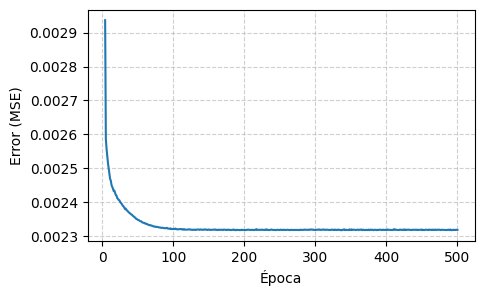
\includegraphics[width=\linewidth]{Images/error0a500.png}
        \caption{Todas las épocas}
    \end{subfigure}
    \vspace{0.55cm} % espacio vertical
    % Segunda subfigura
    \begin{subfigure}{0.65\textwidth}
        \centering
        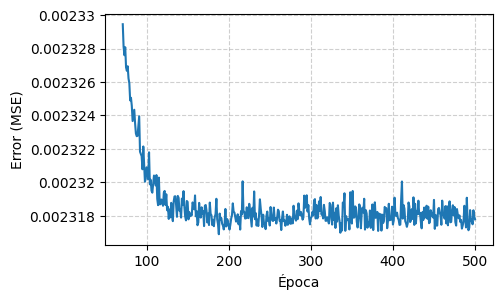
\includegraphics[width=\linewidth]{Images/error70a500.png}
        \caption{Desde la época 70.}
    \end{subfigure}
    \vspace{0.55cm}
    % Tercera subfigura
    \begin{subfigure}{0.65\textwidth}
        \centering
        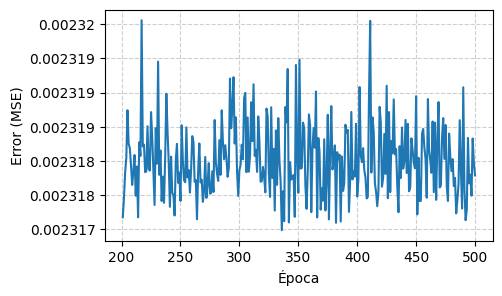
\includegraphics[width=\linewidth]{Images/error200a500.png}
        \caption{Desde la época 200.}
    \end{subfigure}
    \caption{Evolución del error de entrenamiento en función de las épocas para la configuración A15. En (a) vemos el entrenamiento completo, mientras que en (b) y (c) tenemos un acercamiento a la sección final del mismo.}
    \label{fig:tres_errores_train}
\end{figure}

En la figura se ve claramente como primero hay una reducción rápida y pronunciada del error, indicando que el modelo aprende los patrones principales de manera eficiente. La convergencia es notablemente rápida, alcanzando valores cercanos al mínimo antes
de la época $100$. Luego, durante las épocas intermedias, el error continúa disminuyendo pero a un ritmo considerablemente menor, sugiriendo un refinamiento gradual de los pesos del modelo. Esta fase muestra la típica meseta de aprendizaje donde las mejoras incrementales requieren más tiempo de procesamiento.

En la fase final ($200$ a $500$ épocas), el error se estabiliza en valores muy bajos con fluctuaciones menores, sugiriendo que el modelo ha alcanzado un equilibrio, o al menos un mínimo local. Este patrón de convergencia parece indicar que entrenamientos tan largos, aunque garantizan convergencia completa, incluyen un número considerable de épocas redundantes. La configuración A16, idéntica pero con solo $70$ épocas, logra rendimiento prácticamente equivalente, validando esta hipótesis y demostrando la eficiencia de entrenamientos más cortos para arquitecturas bien diseñadas.

\titulito{Visualización de los filtros sobre el conjunto de test}

Vamos a mostrar ahora cómo se ven algunos de los modelos entrenados sobre imágenes del conjunto de test, el cual, recordemos, se compone de imágenes artificiales creadas de la misma manera que el dataset de entrenamiento.

En la figura \ref{fig:imtest_A15} podemos ver el modelo A15, que es el de menor error de testeo, aplicado a una imagen.  El modelo demuestra una capacidad notable para aprender y reproducir los niveles de grises de la imagen original, logrando una reducción efectiva del ruido \emph{speckle}. Sin embargo, se observa que el autoencoder tiende a generar ciertos patrones que no están presentes en la imagen original.

\begin{figure}[htbp]
    \centering
    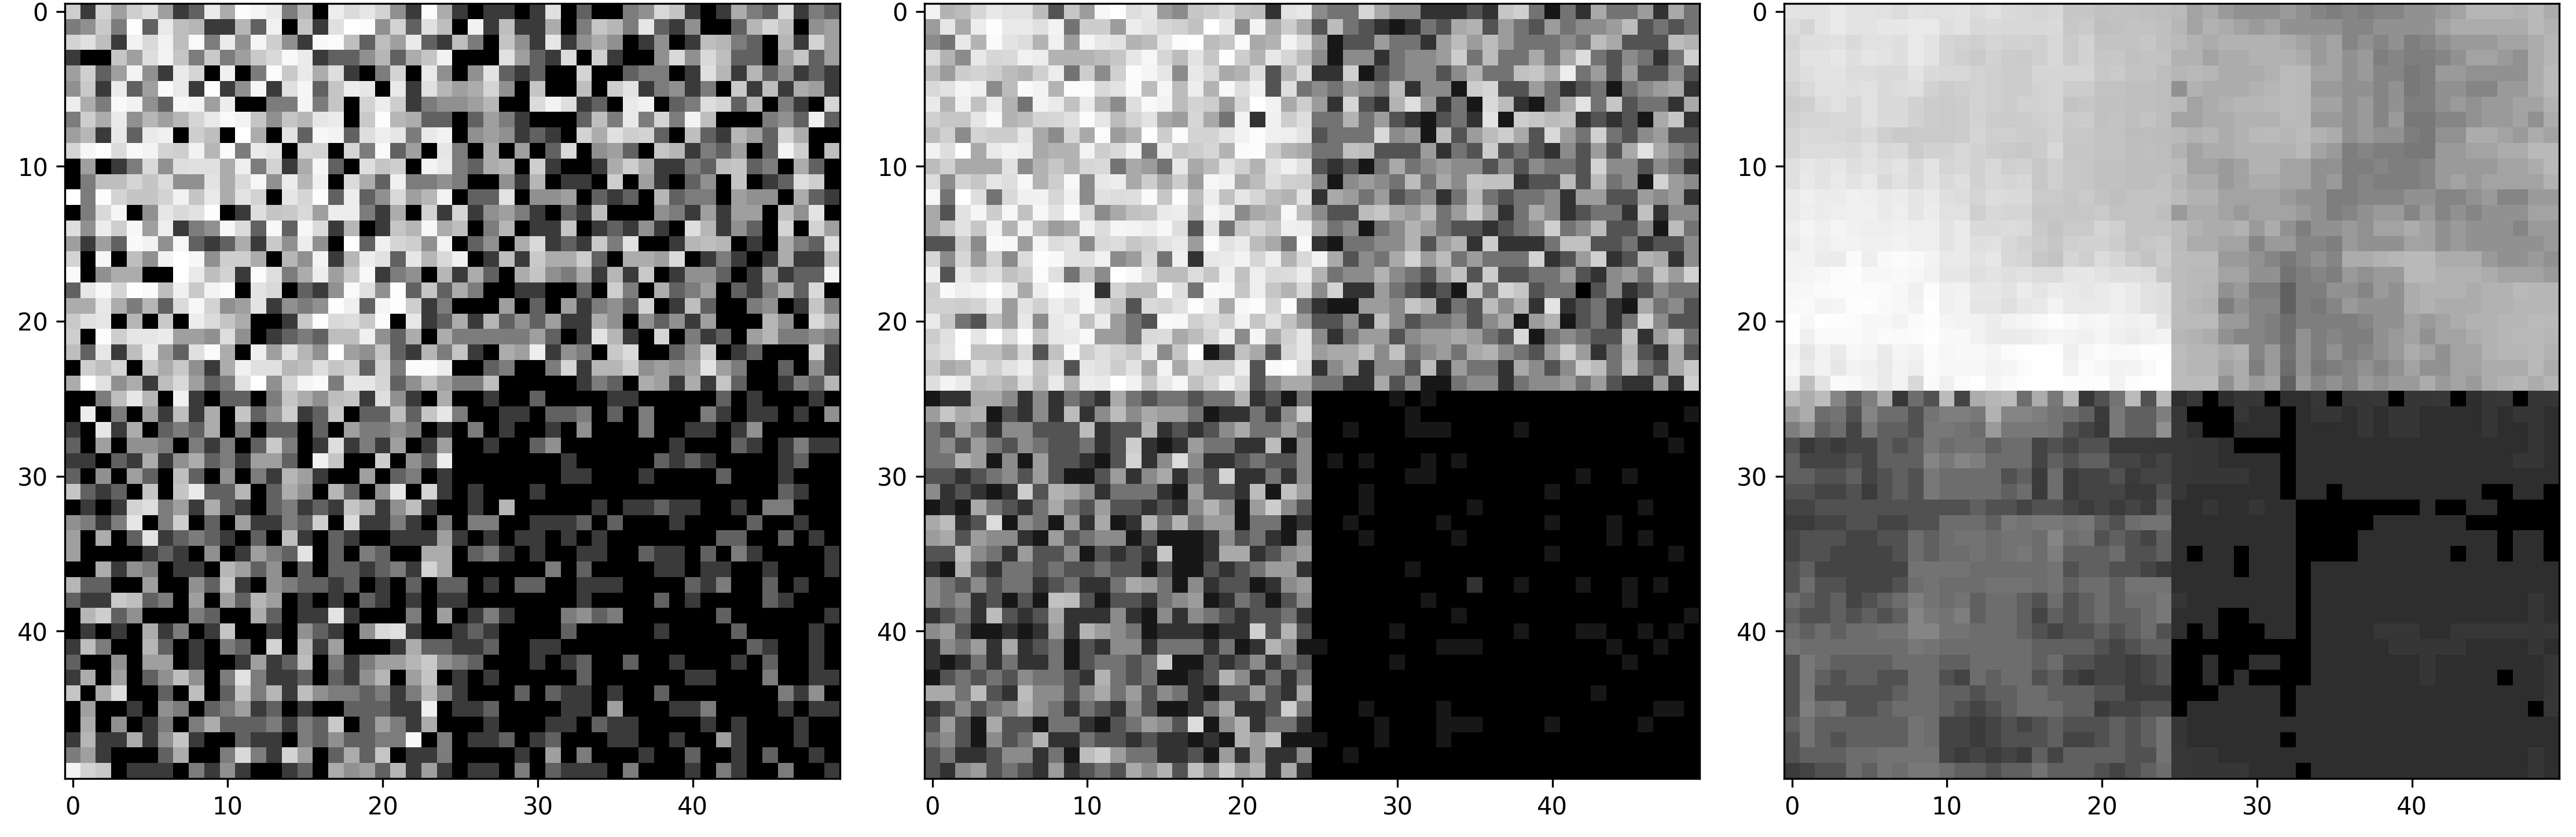
\includegraphics[height=4.5cm]{Images/imtest_A15.png}
    \caption{Imagen de ejemplo ilustrando el filtro A15 aplicado a una imagen del dataset de test. A la derecha está la imagen con ruido \emph{speckle}, la entrada de la red. En el centro está la imagen limpia, el target. A la izquierda está la salida de la red. Todas las imágenes están ecualizadas.}
    \label{fig:imtest_A15}
\end{figure}

Este comportamiento es esperable dado que las redes convolucionales procesan la información teniendo en cuenta que la entrada es una imagen bidimensional, donde la proximidad espacial entre píxeles es un factor determinante. Esta característica hace que el modelo sea sensible a las relaciones de vecindad entre píxeles y tienda a imponer cierta estructura espacial en la reconstrucción, aunque a veces esta no exista originalmente.

La principal limitación observada es la dificultad del modelo para reconocer y preservar adecuadamente la componente aleatoria del \emph{backscatter}. Recordemos que lo describimos como una variable aleatorio con distribución $\Gamma^{-1}$. Mientras que el autoencoder maneja eficientemente los niveles de gris y las estructuras coherentes de la imagen (como los bordes entre particiones), presenta mayor dificultad para distinguir entre el ruido \emph{speckle} que debe eliminarse y la textura natural inherente al \emph{backscatter}, que debería preservarse. Queremos destacar que este comportamiento consistente en todas las arquitecturas.

Veamos ahora en la figura \ref{fig:imtest_A16} el ejemplo de la arquitectura A16, que es idéntica a la A15 salvo que con menos épocas de entrenamiento ($500$ épocas de A15 contra tan solo $70$ de A16). Los resultados obtenidos son notablemente similares a los del modelo A15, lo cual era esperable considerando que ambas arquitecturas presentaron errores de testeo comparables, siendo el de A15 apenas mejor.

\begin{figure}[htbp]
    \centering
    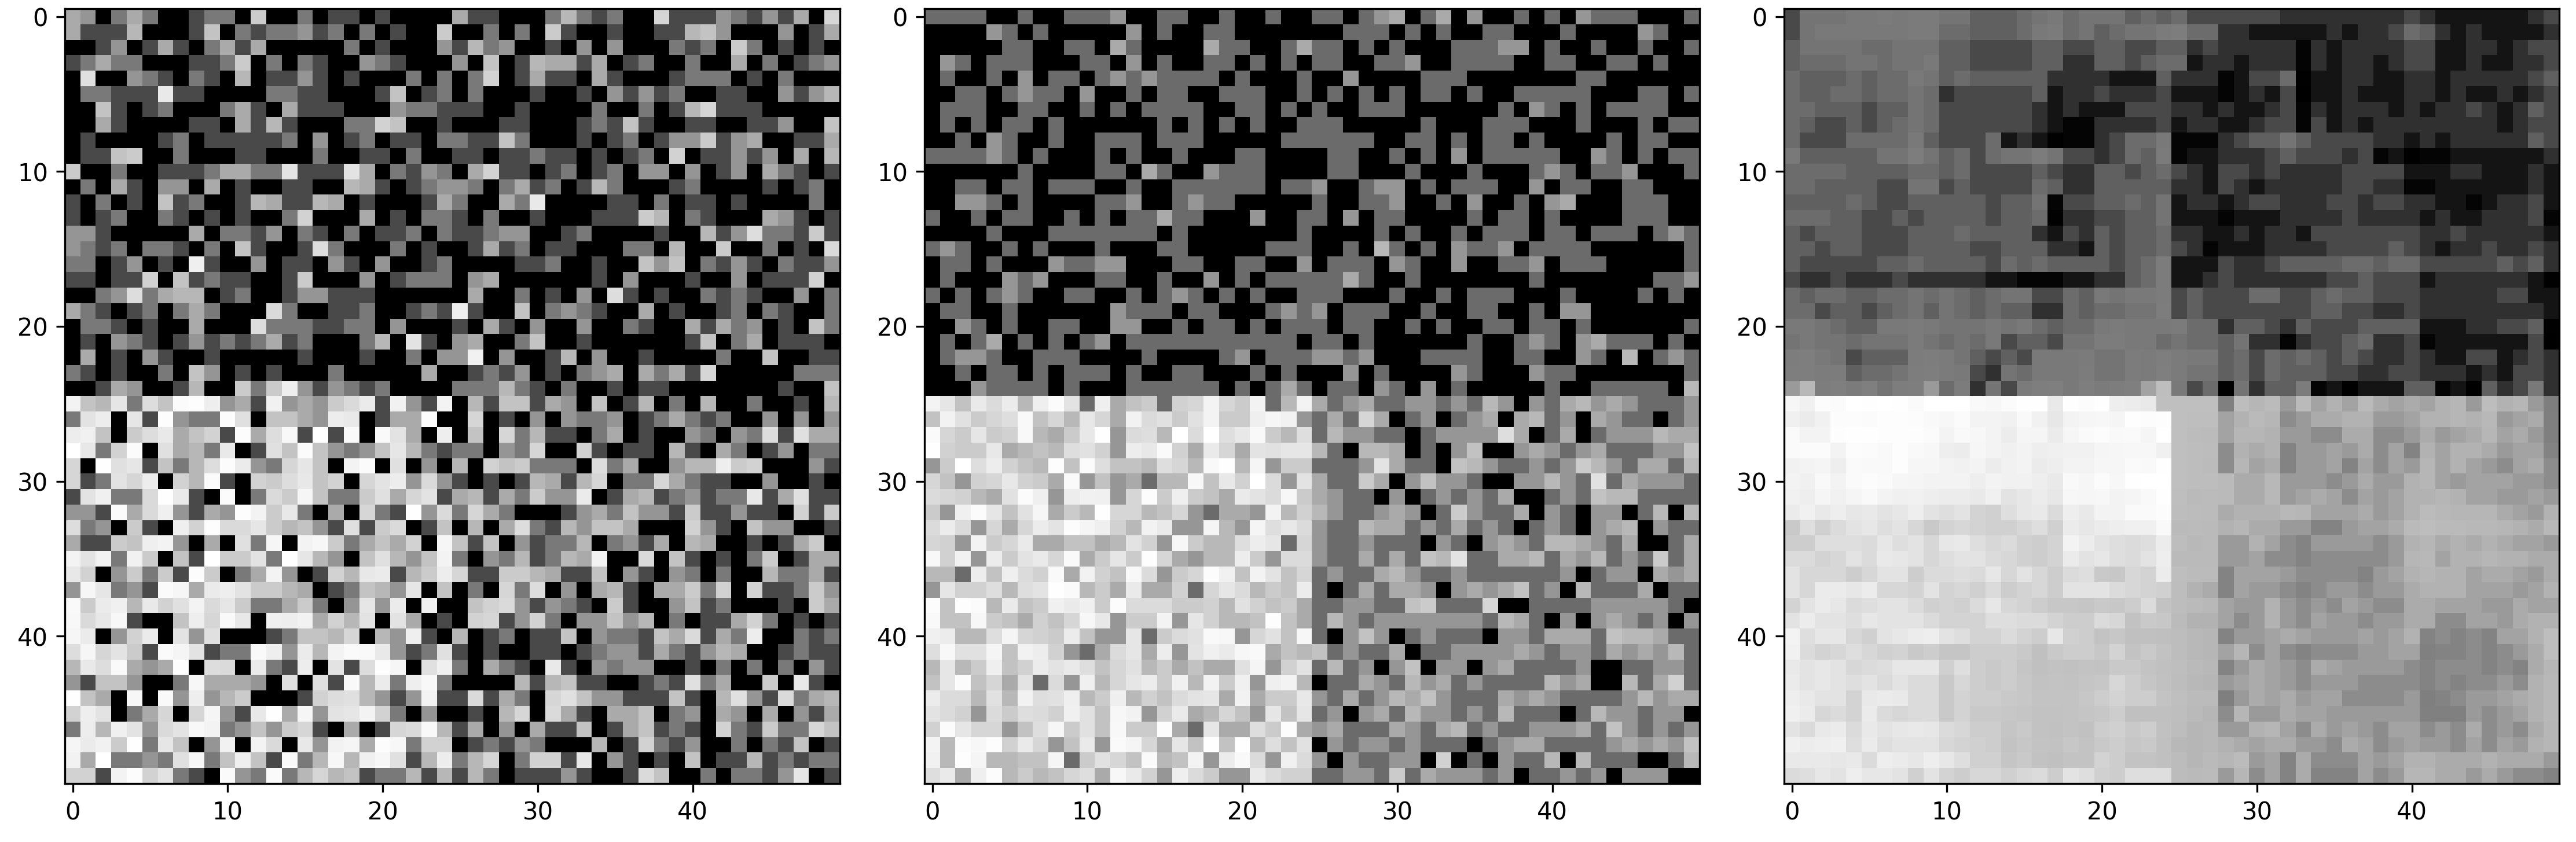
\includegraphics[height=4.5cm]{Images/imtest_A16.png}
    \caption{Imagen de ejemplo ilustrando el filtro A16 aplicado a una imagen del dataset de test. A la derecha está la imagen con ruido \emph{speckle}, la entrada de la red. En el centro está la imagen limpia, el target. A la izquierda está la salida de la red. Todas las imágenes están ecualizadas.}
    \label{fig:imtest_A16}
\end{figure}

La principal diferencia observable radica en la calidad de las estructuras generadas en las zonas homogéneas. En el modelo A16, estas estructuras aparecen ligeramente más toscas y menos suavizadas que en A15, presentando una textura algo más irregular.

Este comportamiento sugiere que el proceso de aprendizaje del autoencoder sigue una progresión específica: durante las primeras épocas de entrenamiento (en las primeras 70, o incluso antes), el modelo adquiere rápidamente la capacidad de entender los niveles de grises y las características más evidentes de la imagen, como los bordes de las particiones. Las épocas adicionales de entrenamiento se dedican principalmente a un proceso de refinamiento, donde el autoencoder ajusta los detalles finos para generar transiciones más suaves y estructuras más regulares.

Por último, en la imagen \ref{fig:imtest_A20} tenemos una visualización de los resultados de la arquitecura A20. Elegimos esa en particular por ser una configuración que utiliza distintas particiones en su dataset de entrenamiento. De hecho, en la figura se observa el filtro aplicado a dos imágenes con particiones distintas.

\begin{figure}[htbp]
    \centering
    
    \begin{subfigure}[b]{\textwidth}
        \centering
        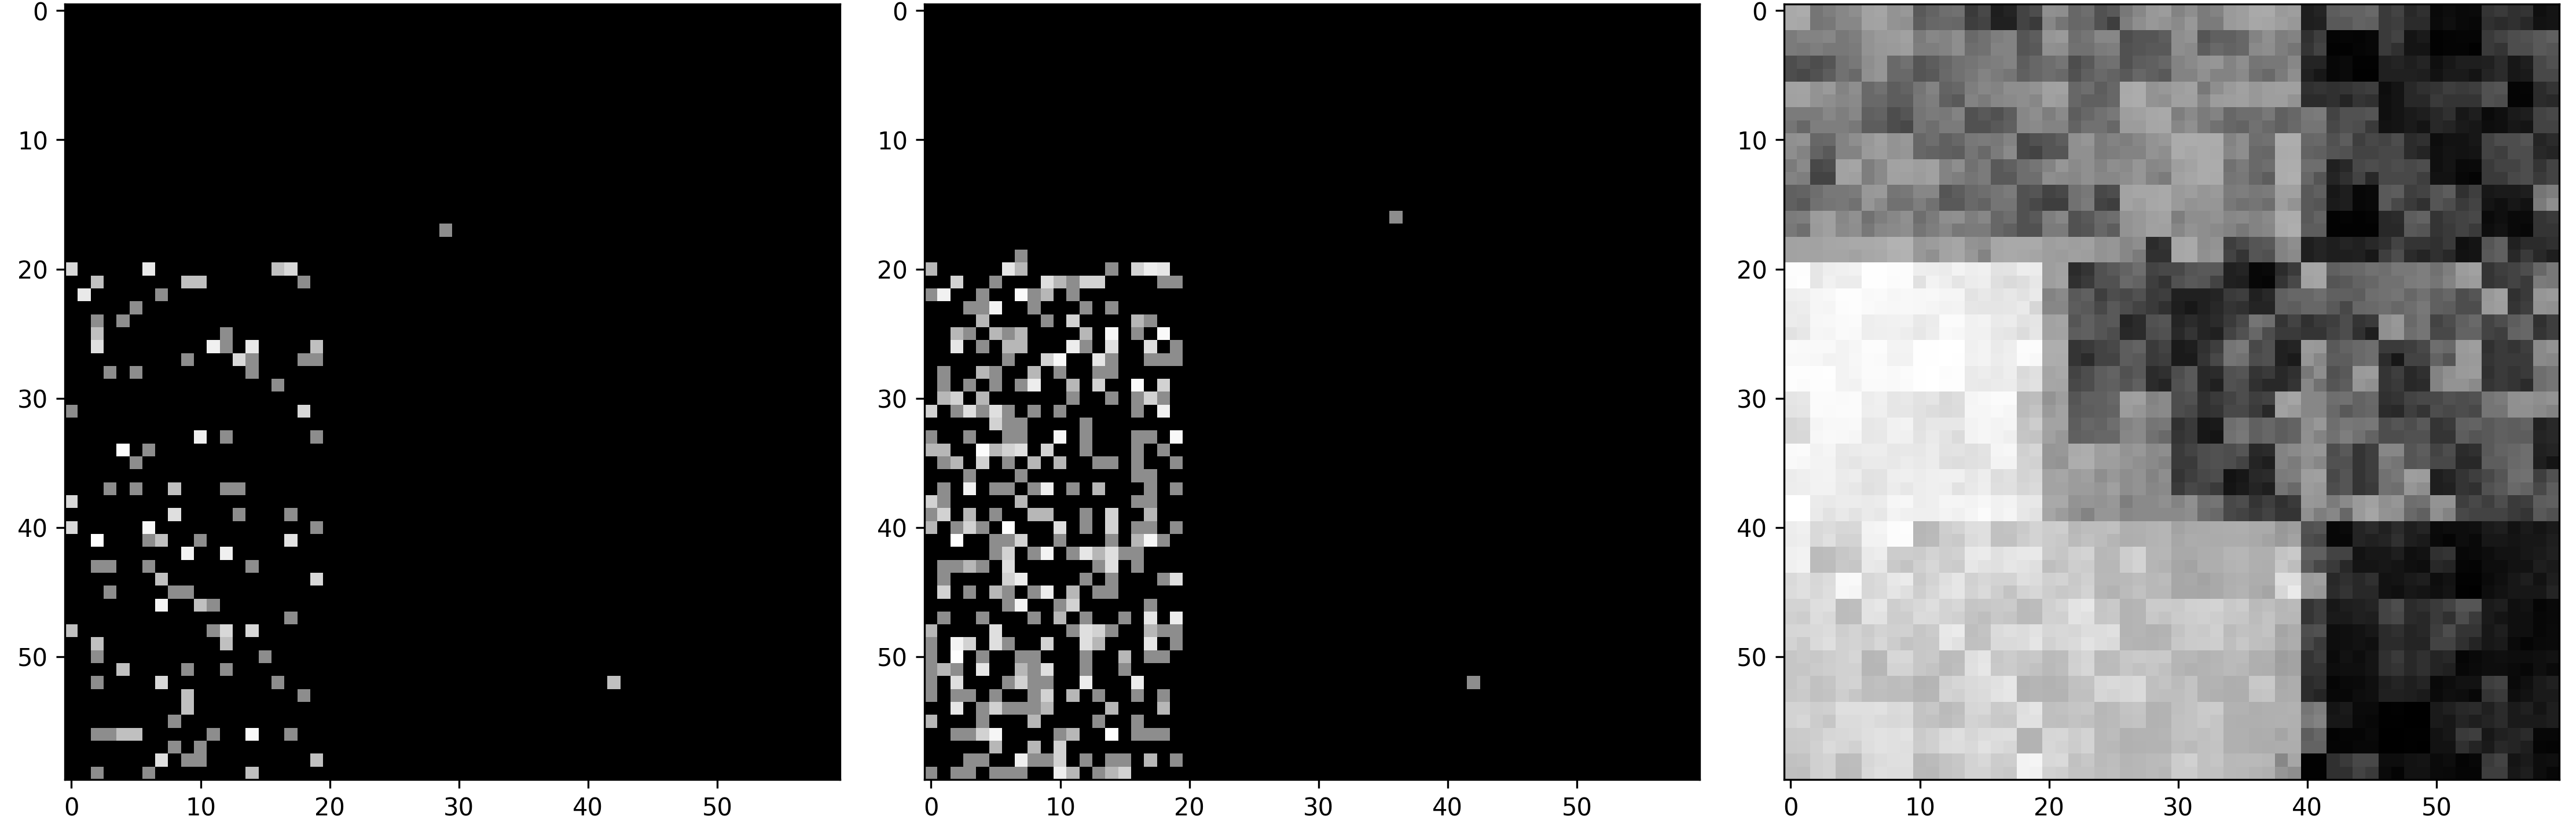
\includegraphics[width=0.9\textwidth]{Images/imtest_A20_1.png}
        \caption{Ejemplo de una imagen con partición de $3\times 3$.}
        \label{fig:imtest_A20_1}
    \end{subfigure}
    
    \vspace{0.5cm} % Espacio entre las subfiguras
    
    \begin{subfigure}[b]{\textwidth}
        \centering
        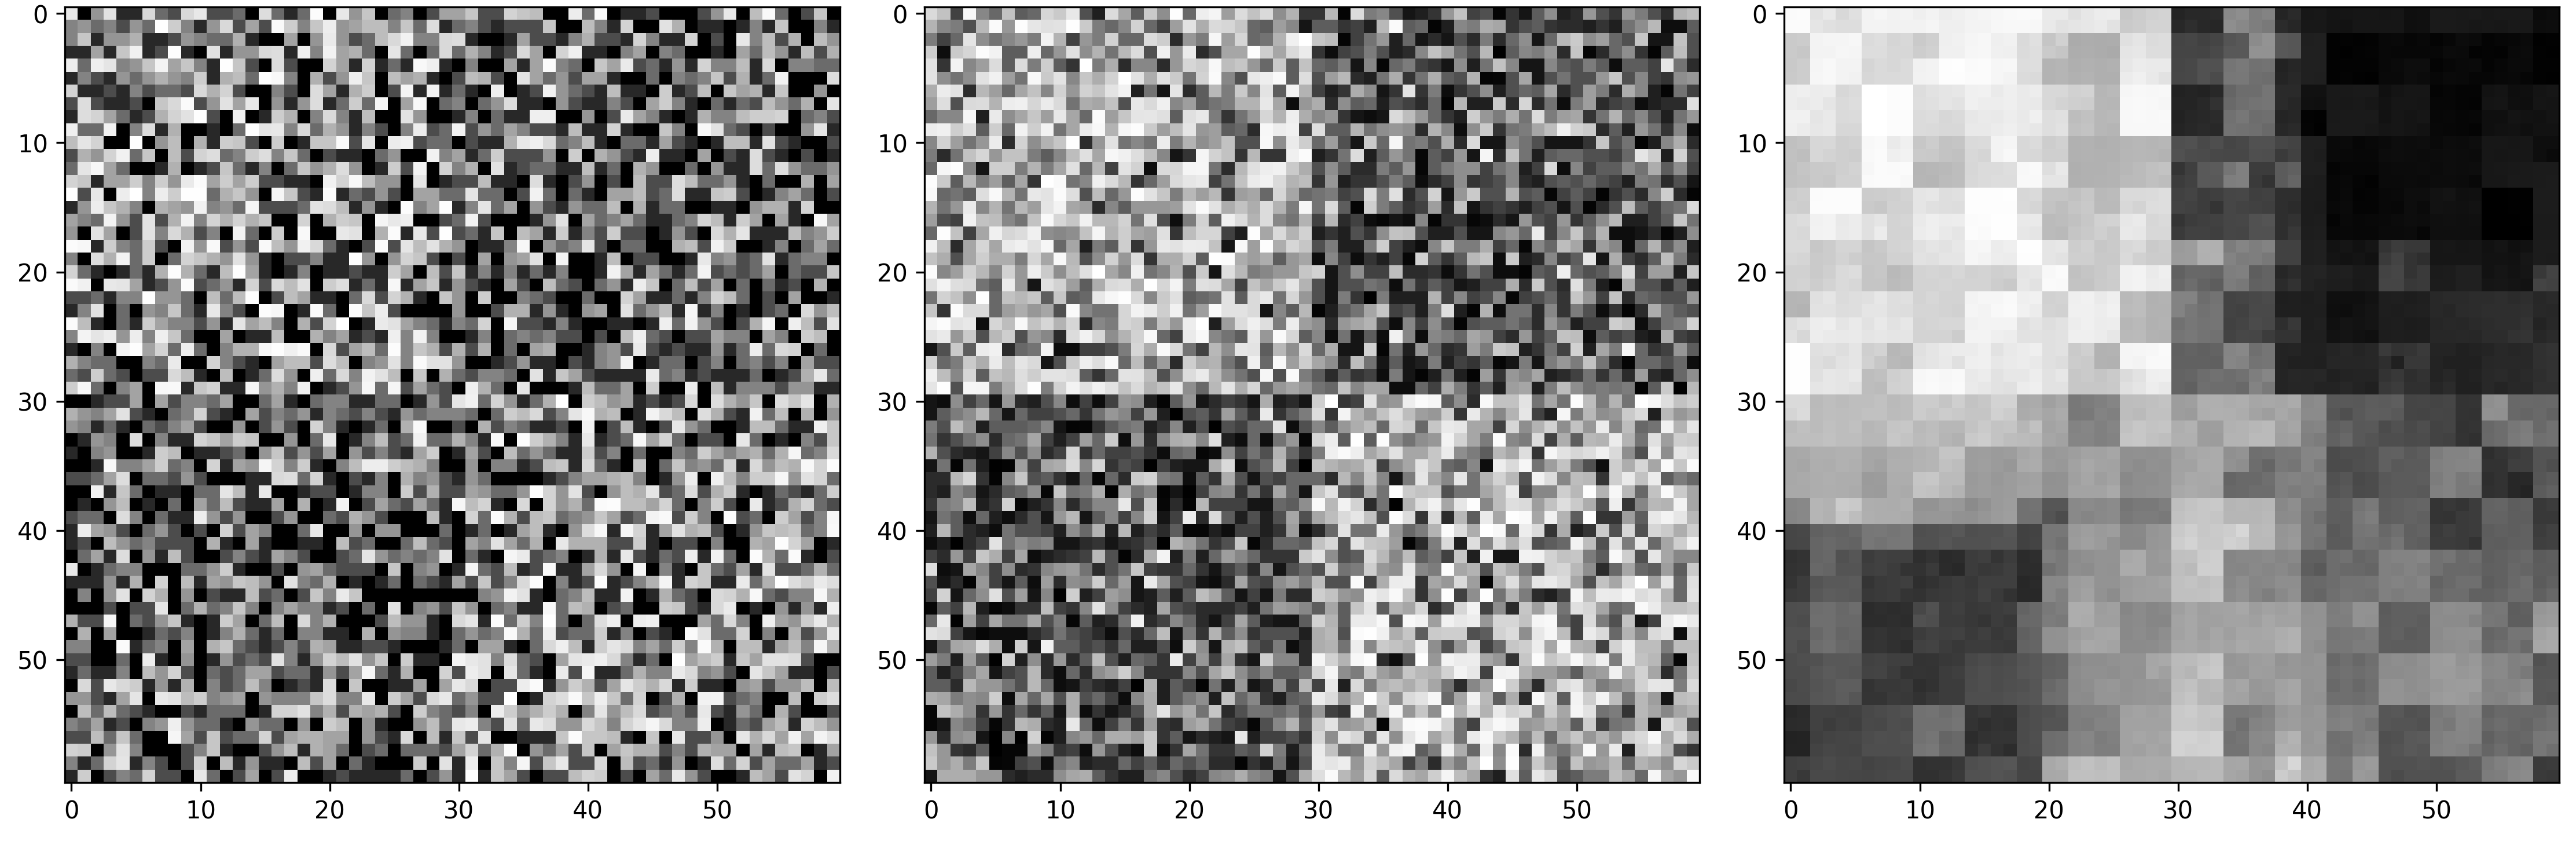
\includegraphics[width=0.9\textwidth]{Images/imtest_A20_2.png}
        \caption{Ejemplo de una imagen con partición de $2\times 2$}
        \label{fig:imtest_A20_2}
    \end{subfigure}
    
    \caption{Imagenes de ejemplo ilustrando el filtro A20 aplicado a una imagen del dataset de test. Tanto en (a) como en (b), a la derecha está la imagen con ruido \emph{speckle}, la entrada de la red. En el centro está la imagen limpia, el target. A la izquierda está la salida de la red. Todas las imágenes están ecualizadas.}
    \label{fig:imtest_A20}
\end{figure}

Visualmente podemos observar que el filtro A20 produce resultados menos prolijos que las arquitecturas A15 y A16 previamente analizadas. Las zonas que deberían presentar características homogéneas aparecen más manchadas y con mayor irregularidad en la textura, mostrando una calidad de suavizado inferior comparada con los modelos anteriores.

Sin embargo, este comportamiento es esperable, considerando que le estamos imponiendo una mayor complejidad al modelo al proporcionarle imágenes con estructuras diversas durante el entrenamiento. Esta variabilidad estructural en el dataset representa un desafío adicional para el autoencoder, que debe aprender a generalizar patrones de limpieza de ruido \emph{speckle} a través de diferentes configuraciones espaciales y características de imagen.

Esta aparente pérdida en el resultado es, en realidad, el precio que pagamos por ganar flexibilidad y capacidad de generalización. Esperamos que esta mayor robustez del modelo se traduzca en un mejor desempeño cuando se enfrente a imágenes SAR reales, cuyas estructuras son inherentemente menos organizadas y rígidas que las imágenes sintéticas utilizadas en el entrenamiento. La capacidad del modelo A20 para manejar esta diversidad estructural debería resultar en una mayor adaptabilidad a las condiciones variables y complejas presentes en datos SAR del mundo real.

\subsection{Aplicación del modelo a imágenes reales}

\textcolor{red}{
\begin{itemize}
    \item poner imágenes.
    \item voy a tener que decir que es una debilidad de entrenar con imagenes sinteticas, el hecho de que no aprende la estructura de una imagen cualquiera, sino que parece aprender los cuadrantes. poner que por eso despues propusimos entrenar con imagenes reales.
\end{itemize}
}

\subsection{Métodos estadísticos de medición de la calidad del filtro}

\textcolor{red}{
\begin{itemize}
    \item quizas una tabla con los errores de 1er y 2do orden?
    \item decir que usamos g=30 para el estadístico de segundo orden.
\end{itemize}
}

\subsection{Comparación con otros filtros}

\textcolor{red}{
\begin{itemize}
    \item Comparación con el filtro de Lee. No importa tanto que mis autoencoders sean mejores que Lee, sino que compitan.
    \item NOTA PARA MI: me falta correr errores de comparacion con otros filtros para A14 (el quality filters)
\end{itemize}
}

\section{Modelos entrenados con imágenes reales}
